\documentclass{article}
\usepackage[utf8]{inputenc} %кодировка
\usepackage[T2A]{fontenc}
\usepackage[english,russian]{babel} %русификатор 
\usepackage{mathtools} %библиотека матеши
\usepackage[left=1cm,right=1cm,top=2cm,bottom=2cm,bindingoffset=0cm]{geometry} %изменение отступов на листе
\usepackage{amsmath}
\usepackage{graphicx} %библиотека для графики и картинок
\graphicspath{}
\DeclareGraphicsExtensions{.pdf,.png,.jpg}
\usepackage{subcaption}
\usepackage{pgfplots}
\usepackage{listings}

\begin{document}
% НАЧАЛО ТИТУЛЬНОГО ЛИСТА
\begin{center}
    \Large
   
    \vspace{0.5cm}
    \large
  
    \vspace{1cm}
    \Large
    \textbf{Java repeat course} \\
   
    \large
    \vspace{8cm}

    \begin{minipage}{.33\textwidth}
    \end{minipage}
    \hfill
    \begin{minipage}{.4\textwidth}
    
        
    \end{minipage}
    \vfill
Санкт-Петербург\\ 2023 г.
\end{center}

% КОНЕЦ ТИТУЛЬНОГО ЛИСТА 
\newpage



\section{Основы}
\tiny
\begin{minipage}{.3\textwidth}
    \textbf{Множественное наследование в Java}\\
    Существенное различие между классами и интерфейсами заключается в том, 
    что классы могут иметь поля, в то время как интерфейсы - нет. 
    Кроме того, можно создать экземпляр класса для создания объекта, что нельзя 
    сделать с интерфейсами. Объект сохраняет свое состояние в полях, которые определены в классах. 
    Одна из причин, по которой язык программирования Java не позволяет расширять более одного класса - 
    избегание проблем множественного наследования состояния, которое заключается в 
    возможности наследовать поля из нескольких классов.
\end{minipage}
\hfill
\begin{minipage}{.3\textwidth}
    \textbf{Модификаторы доступа}
    Модификаторы уровня доступа определяют, могут ли другие классы использовать определенное поле или вызывать определенный метод.
    Существует два уровня контроля доступа: top level — public or default; member level — public, private, protected, default;\\
    private - виден в пределах класса\\
    protected - виден в пределах родительского класса и его наследников в рамках одного пакета\\
    default(package-private) - виден в пределах пакета, в котором находится\\
    public - виден за пределами пакета, в котором находится\\
\end{minipage}
\hfill
\begin{minipage}{.3\textwidth}
    \textbf{Программа, выводящая список аргументов командной строки}\\
    import java.util.Arrays;
\\
    public class Main \{\\
        public static void main(String[] args) \{\\
            System.out.println(Arrays.toString(args));\\
        \}\\
    \}
    
\end{minipage}
\\ \\

\begin{minipage}{.3\textwidth}
    \textbf{Модель состояний потока в Java}\\
    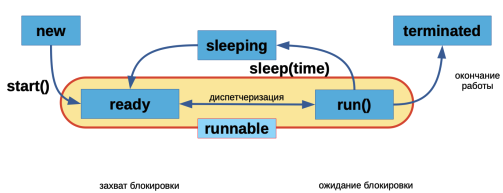
\includegraphics[width=.9\textwidth]{model}
    
\end{minipage}
\hfill
\begin{minipage}{.3\textwidth}
    \textbf{Виды полиморфизма в Java}\\
    Полиморфизм подтипов - достигается через 
    наследование и реализацию интерфейсов. Позволяет объектам одного класса быть 
    использованными объектами другого класса через общий суперкласс или интерфейс. 
    Это включает в себя использование переопределенных методов.\\
    Полиморфизм параметров - позволяет 
    создавать generic классы и методы, которые могут работать с разными типами 
    данных.\\
    Полиморфизм перегрузки - позволяет создавать несколько методов с одинаковыми именами в 
    классе, но с разными параметрами. Выбор метода для вызова основывается на сигнатуре метода.\\
    Полиморфизм интерфейсов - связан с использованием интерфейсов в Java. 
    Классы могут реализовывать интерфейсы, и объекты классов могут быть рассматриваемыми как объекты интерфейсов.
    
\end{minipage}
\hfill
\begin{minipage}{.3\textwidth}
    \textbf{Программа, выводящая текущие время и дату}\\
    import java.time.LocalDateTime;\\
    import java.time.ZoneId;\\
    import java.time.format.DateTimeFormatter;\\

public class Main \{\\
    public static void main(String[] args) \{\\
        DateTimeFormatter formatter = DateTimeFormatter.ofPattern("Год: y; Месяц: M; День: d; Время: H-m-ss");\\
        System.out.println(formatter.format(LocalDateTime.now(ZoneId.of("Europe/Moscow"))));\\
    \}
\}
\end{minipage}
\\ \\



\begin{minipage}{.3\textwidth}
    \textbf{Примитивные и ссылочные типы}\\
    Примитивные типы: 
byte(8 bit),
short(16 bit),
int(32 bit),
long(64 bit),
float(32-bit),
double(64-bit),
bool(true/false),
char(16-bit unsigned).\\
Ссылочные типы: class types, interface types, type variables, array types
    
\end{minipage}
\hfill
\begin{minipage}{.3\textwidth}
    \textbf{Блоки инициализации}\\
    Существуют два вида блоков инициализации:\\
    Статический - используется для инициализации статических полей и 
    выполняется всего один раз при первом обращении к классу\\
    Нестатический - используется для инициализации нестатических переменных и 
    выполняется каждый раз при создании нового
    Порядок выполнения блоков при создании нового объекта:
1 - Статический блок инициализации (будет выполнен при первом создании объекта и если не было обращений прежде в классу);
2 - Родительский конструктор через вызов super;
3 - Нестатический блок инициализации;
4 - Тело конструктора
\end{minipage}
\hfill
\begin{minipage}{.3\textwidth}
    \textbf{Программа, записывающая строку "Hello!" в файл world.txt}\\
        import java.io.FileWriter;\\
        import java.io.IOException;\\
        
        public class WriteToFile \{\\
            public static void main(String[] args) \{\\
                String fileName = "world.txt";\\
        
                try \{\\
                    FileWriter writer = new FileWriter(fileName);\\
                    String content = "Hello!";\\
                    writer.write(content);\\
                    writer.close();\\
        
                    System.out.println("succses");\\
                \} catch (IOException e) \{\\
                    System.err.println("err" + e.getMessage());\\
                \}
            \}
        \}

\end{minipage}
\\ \\

\begin{minipage}{.3\textwidth}
    \textbf{Классификация потоков ввода/вывода}\\
    Потоки ввода (Input) и вывода (Output) подразделяются на: Байтовые и Символьные\\
    Для взаимодействия с IO существуют базовые классы:\\
    InputStream — поток для чтения байтов (поток ввода)\\
Reader — поток для чтения символов (поток ввода)\\
OutputStream — поток для записи байтов (поток вывода)\\
Writer — поток для записи символов (поток вывода)
    
\end{minipage}
\hfill
\begin{minipage}{.3\textwidth}
    \textbf{Ключевое слово import}\\
    Ключевое слово import используется для импортирования классов, интерфейсов, пакетов и библиотек - 
    это позволяет нам обращаться к классам не по полному имени (со всеми пакетами), 
    а по самому имени.
\end{minipage}
\hfill
\begin{minipage}{.3\textwidth}
    \textbf{Программа, выводящая в консоль количество переданных ей аргументов}\\
    public class Main \{\\
    public static void main(String[] args) \{\\
        System.out.println(args.length);\\
    \}
\}

\end{minipage}
\\ \\

\begin{minipage}{.3\textwidth}
    \textbf{Массивы и коллекции}\\
    Массивы — это простые конструкции фиксированного размера, и поэтому они могут 
    хранить только заданное количество элементов. Массивы встроены в ядро языка Java. 
    Массивы могут хранить элементы определенного типа \\
    Коллекции — могут динамически изменять свой размер, что делает их более гибкими, чем массивы. Существуют базовые коллекции в Java:
List, 
Queue, 
Set, 
Map (но стоит заметить, что Map не является реализацией интерфейса Collection, но является частью фреймворка Collections)
    
\end{minipage}
\hfill
\begin{minipage}{.3\textwidth}
    \textbf{Классы StringBuilder и StringBuffer}\\
    Класс StringBuilder является решением проблемы неизменяемости объектов String - при помощи данного класса 
    можно модифицировать строки, конкатенировать и тд (без создания дополнительного объекта, как это делает String).\\
    StringBuffer - так же позволяет гибко редактировать строки без создания дополнительных объектов, но дополнительно является потокобезопасным и синхронизованным (работает медленнее)
\end{minipage}
\hfill
\begin{minipage}{.3\textwidth}
    \textbf{Программа, записывающая содержимое файла in.txt в файл out.txt}\\
    public class FileCopy \{\\
    public static void main(String[] args) \{\\
        String inputFile = "in.txt";\\
        String outputFile = "out.txt";\\
        try (BufferedReader reader = new BufferedReader(new FileReader(inputFile));\\
             BufferedWriter writer = new BufferedWriter(new FileWriter(outputFile))) \{\\
            String line;\\
            while ((line = reader.readLine()) != null) \{\\
                writer.write(line);\\
                writer.newLine();\\
            \}\\
            System.out.println("успешно");\\
        \} catch (IOException e) \{\\
            System.err.println("Ошибка " + e.getMessage());\\
        \}
    \}
\}

\end{minipage}

\end{document}
